\section{Introduction}
% With the broader coverage of online shopping across people in different ages and occupations, shopping demand varies for specific group of people or at specific period of time. In big companies, the traditional all-in-one shopping business pattern prone to be substituted by multiple business lines serving for people with distinct purposes. For example, 
% \KZ{This para is not well written.
% Go directly to explain what's product categorization and what it means by dynamic taxonomy scenario. No need to beat around the bush. One para on traditional problem and one para on the new problem will do. Now is too long! Don't introduce new names and acronyms at the beginning of the paper, especially the abstract. Use very easy to understand language.} When a broader coverage people embracing online shopping in recent years, numerous sellers swarm into e-commerce platforms with a surge of various kinds of products. 
% While the number of products keeps rising, it poses a bigger challenge for sellers to assign them with category tags and for platforms to manually organize them into category taxonomies as well. 
% Thus e-commerce platforms aim to train a model that automatically categorizes products and provide suggestions for those sellers, in order to improve their user experience.

% Typically product categories are organized into a hierarchical structure and 
Product categorization \cite{ding2002goldenbullet} is a specific text classification task which classifies the products into a pre-defined taxonomy of category nodes, using their description texts such as titles. 
For example, a product named \textit{``Red Wine Flavor Ice Cream $60g \times 6$''} should be categorized into 
% \textit{"Dairy Food $\rightarrow$ Frozen $\rightarrow$ Ice Cream"}.
\verb|Dairy Food| $\rightarrow$ \verb|Frozen| $\rightarrow$ \verb|Ice Cream|.
% It is also a crucial part of product understanding in which the accurate categorization of products further provides guidance for other e-commerce application scenarios, such as the user query navigation or advertisement recommendation. 

\begin{figure}[tbp]
  \centering
  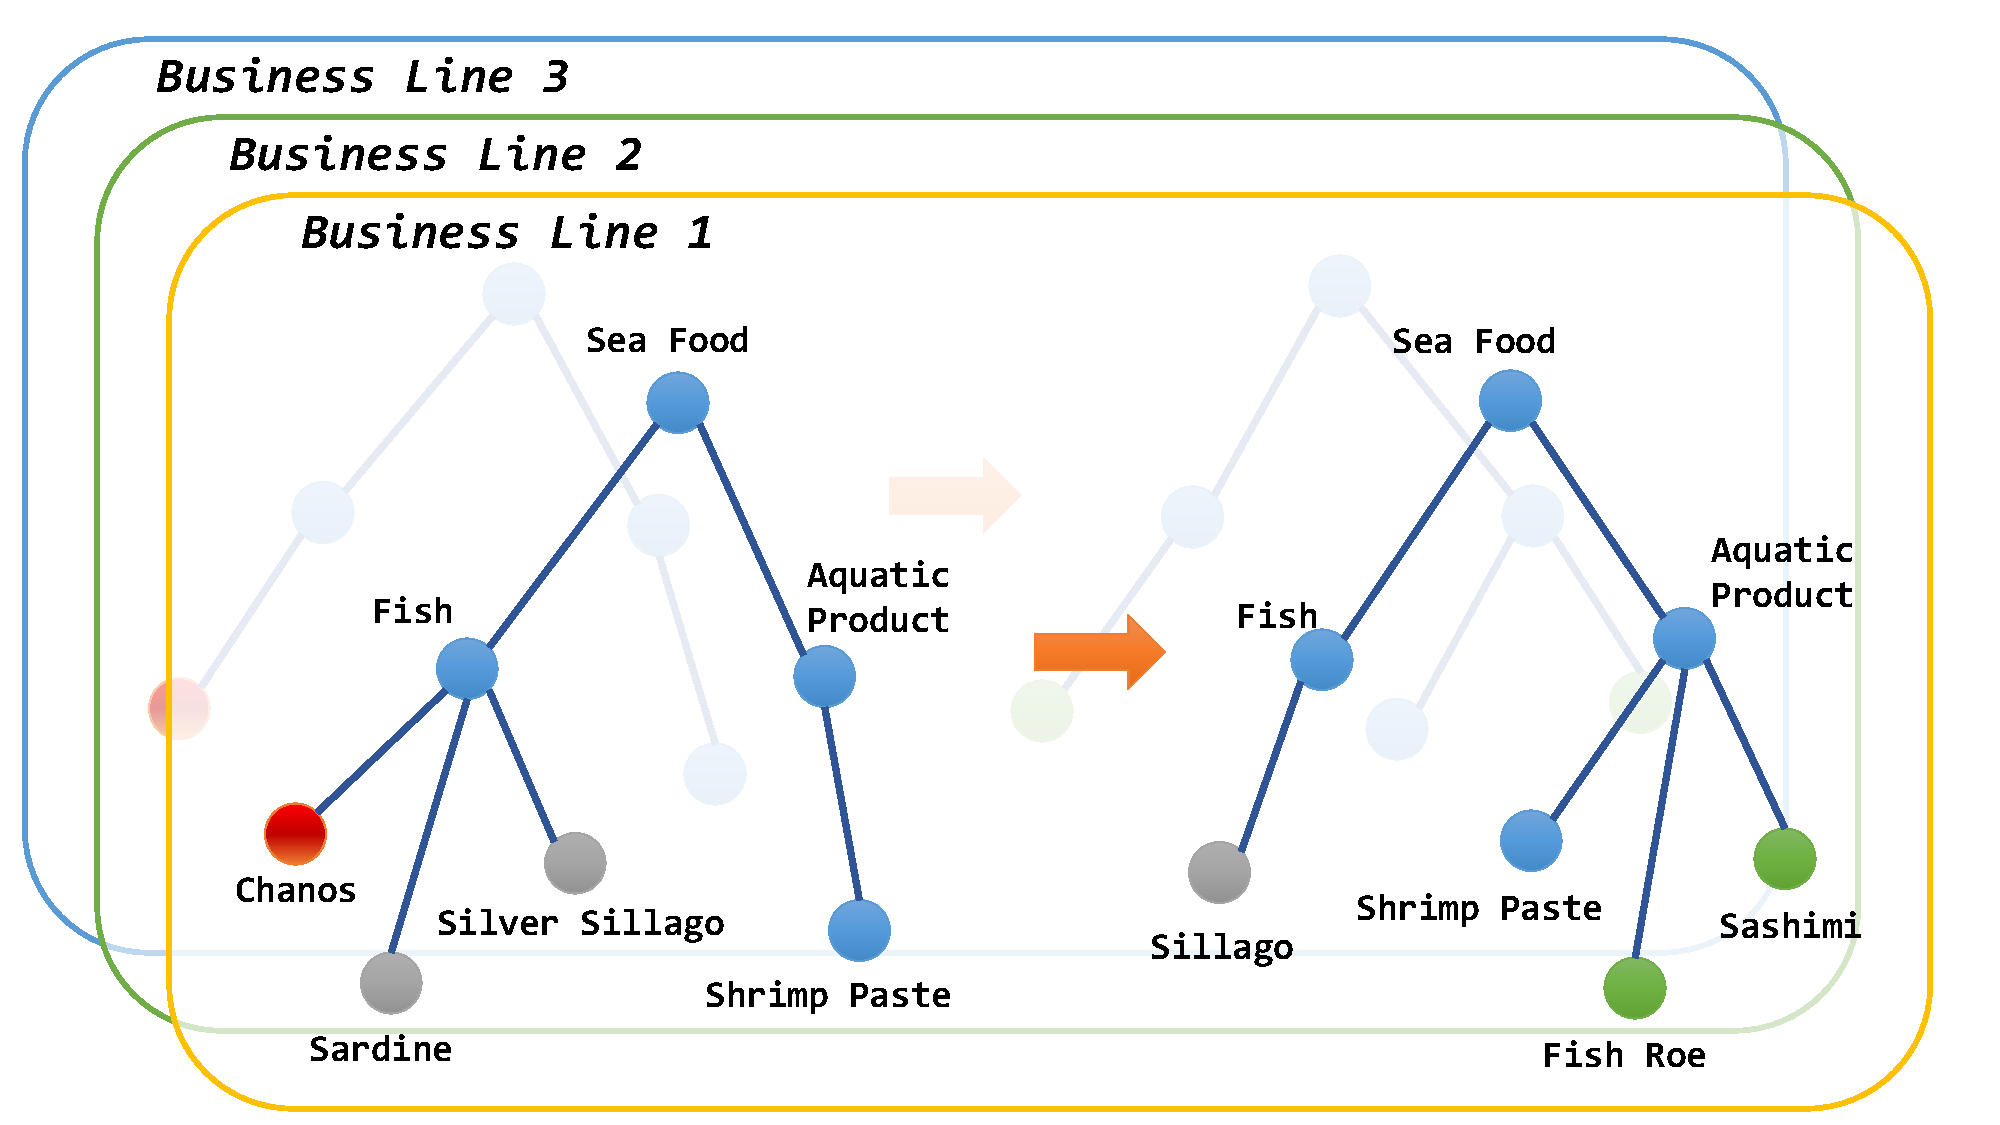
\includegraphics[width=\linewidth]{teaser}
  \caption{An illustration of multiple taxonomies and taxonomy evolving. Multiple taxonomies from different business lines are evolving themselves, where the nodes colored red, grey and green refers to deletion, integration and increment respectively.}
  \label{fig:teaser}
\end{figure}

Unlike vanilla text classification tasks, product categorization in e-commerce scenarios deals with thousands of fine-grained leaf node categories, which is known as the \textbf{large label space} challenge.
% For example in Meituan e-commerce platform, there are an average -- newly uploaded products per day. 
Although plenty of works concentrate on this challenge and formulate it as a multi-class hierarchical classification task with a fixed set of labels~\cite{kozareva2015everyone, cevahir2016large}, they ignore the situation where there exists multiple category taxonomies from different business lines and they will continuously evolve. 

A real world problem that e-commerce platforms (\textit{e.g.,} Amazon and Alibaba) have to deal with is to maintain multiple business lines and their corresponding taxonomies.
% but share a part of similar products. 
These business lines usually cater for different customer demands or fine-grained business domains, for example, some provide fast delivery while others specialize in low price products. 
Multiple lines maintain different category label tree structures, with various depths and distinct literal expressions of tree nodes. Traditional classification approaches are feasible only on separate models for each business line, which is laborious to operate and maintain. 
% In addition, these models trained on specific category structures are incapable of extrapolating to another taxonomy categorization task. 
We name this \textbf{multi-domain taxonomies} challenge.

On the other hand, with the expansion and reorganization of business, the category taxonomy keeps evolving as well. 
As is shown in \figref{fig:teaser}, when a minor business adjustment happens, \verb|Sardine| and \verb|Silver Sillago| are integrated into one category \verb|Sillago|, while \verb|Chanos| is removed and \verb|Fish Roe|, \verb|Sashimi| are added to the taxonomy. 
For conventional approaches, models should be re-trained every time the taxonomy changes, which is too costly. We call this the challenge of \textbf{evolving taxonomy}.

\cut{%%%%%%%%%%% No need the following summary %%%%%
To sum up, challenges behind product categorization of giant e-commerce platforms are listed below.  
% \KZ{These challenges should be illustrated using some lively examples.}

\begin{enumerate}
    \item \textbf{Large label space}, a fundamental challenge that has been well studied in former works. They either use a flat classifier treating all leaf nodes equivalently \cite{yu2012product, ha2016large, das2016large, krishnan2019large, lee2020cbb, yang2020bert}, or follow the hierarchy structure to classify from coarse to fine level nodes \cite{hasson2021category, li2018don}.
    \item \textbf{Multi-domain taxonomies}. This is mostly studied in the multi-task learning paradigm \cite{liu-etal-2019-multi}, which manipulates different tasks with a joint model. However, it lacks the ability to tackle taxonomy evolving.
    \item \textbf{Taxonomy evolving}. Authors in \cite{xu2019open} formulated an open-world learning problem in which a model should reject unseen classes and learn to recognize new classes incrementally. Nonetheless, conditions when classes are integrated or divided apart are ignored in their work.
\end{enumerate}
}%%%%%%%%%%%%%%%

% To our best knowledge, there is no solution in e-commerce that could apply for all the three challenges.
Derived from the above scenarios in production, we define the problem in which the above three challenges are considered simultaneously as Dynamic Multi-Domain Product Categorization (DMPC) problem. 
% In this work, we propose a unified framework named \textit{Taxonomy-agnostic Label Retrieval (TaLR)} to solve the problem above.
Intuitively, we consider to reformulate such dynamic classification problem as category label retrieval problem in order to jointly circumvent the above issues. However, it is non-trivial to obtain both product titles and category label representations ensuring both accuracy and efficiency. 

Considering the rich semantic information included in category names, we further solve this label retrieval problem following the sentence matching task by calculating semantic similarity between product titles and category label texts, in which the label with closest textual meaning to target product title is treated as the predicted category. 
This reformulation is especially beneficial for \textbf{evolving taxonomy} challenge when pretrained language models are incorporated, while the knowledge from \textbf{multi-domain taxonomies} can be jointly leveraged as well.
For example, in \figref{fig:teaser}, despite the integration of \verb|Sardine| and \verb|Silver Sillago| into \verb|Sillago|, their textual meanings are barely drifted, and the corresponding semantics are remained. 
Furthermore, a unified semantic-matching-based framework can recognize the internal connections of new product names and new classes (like \verb|Fish Roe| and \verb|Sashimi|) with the aid of the knowledge from pretrained language models or training data from other domain taxonomies. Even for an extreme condition of taxonomy evolving that a brand new taxonomy from other companies or business lines emerges, it may share certain concepts with the existing taxonomy, which could be captured in textual semantics as well. 

However, pure sentence matching methods might be insufficient for accurate product categorization when some hidden rules are ignored.
For example, \textit{``Haagen-Dazs Red Wine Flavor''} might be wrongly categorized into \verb|Alcoholic Drinks| $\rightarrow$ \verb|Wine| $\rightarrow$ \verb|Red Wine| instead of the correct \verb|Dairy Food| $\rightarrow$ \verb|Frozen| $\rightarrow$ \verb|Ice Cream|, in that the key word \textit{``Red Wine''} possibly misleads sentence matching models to a skewed direction. 
We thus propose a rule-based unit to provide complementary information besides textual matching.
% We can also return the predicted top-$k$ categories as the suggestions for product sellers.
While the large label space will pose bigger challenge for one-vs-all retrieval models, we adopt bi-encoder BERT \cite{devlin-etal-2019-bert} to pursue the inference time efficiency and recall of category label candidates, and further followed by a cross-encoder BERT to ensure sentence matching precision.
Also, to make full use of the mutual interactions between the product title and the category name pair-wisely in their representative semantic space, we use the contrastive information delivered by both inter-class and intra-class product titles.
% Since conducting one-vs-all similarity measurement for a product title to the full set of labels in the extremely large space is highly time consuming, 
Accumulating all the above motivations, we design a two-stage \textit{Retrieval-Reranking} pipeline inspired by industrial recommendation systems and name it as \textit{Taxonomy-agnostic Label Retrieval (TaLR)} framework.
% The \textit{Retrieval} stage has two components, the vector-based retrieval model and the rule-based retrieval algorithm. We also adopt several fusion strategies combining them two to generate the candidate category names which are further processed in the next stage.
% The \textit{Reranking} stage captures more precise semantic relatedness of product titles and candidate category names using a BERT cross-encoder binary classifier. 

We conduct experiments on three distinctly annotated product categorization datasets with independent taxonomies and evaluate our framework using accuracy score. Results show the advantages of our proposed \textit{TaLR} framework. It outperforms the baseline classifiers trained on each task respectively. Meanwhile, it sustains accuracy under several taxonomy evolving scenarios and is able to extrapolate to the incoming unseen taxonomy in a zero-shot manner without re-training.
% \TODO{add time consuming if there is}
Moreover, the two-stage \textit{TaLR} exhibits the advantage on both accuracy and time efficiency over the simple cross-encoder BERT \textit{Reranking} approach. 

In conclusion, our contributions are:
% \KZ{I would say your main contributions are: i) using one model for all tax is better than using separate models for each tax; ii) using the retrieval then reranking framework is better (both accuracy and speed) than one-off classification; iii) other small tricks.} 
\begin{itemize}
    % \item We address three challenges in Dynamic Multi-Domain Product Categorization (DMPC) which are \KZ{urgently to be solved}, and propose the  \textit{Taxonomy-agnostic Label Retrieval (TaLR)} \TODO{TARR} framework as an unified solution. \KZ{This item is not very useful. U just give a name of the framework which doesn't say what really is the contribution. Again, not refutable!}
    \item We propose a unified \textit{Taxonomy-agnostic Label Retrieval (TaLR)} framework for multi-domain product categorization, which jointly leverages knowledge from multiple domain, 
    while incurs low operation \& maintenance cost and gives rise to low response latency. (\secref{sec:all res}, \secref{sec:time cons})
    % \item We leverage the contrastive information from inter-class and intra-class product titles to effectively boost the product understanding  of the model. 
    \item Our \textit{TaLR} framework is generalized to handle evolving taxonomies and emerging new taxonomies, 
    where its zero-shot performance is even better than few-shot baselines. (\secref{sec:evolve res}, \secref{sec:new tax})
    % and to give good performance on zero-shot scenarios. (\secref{sec:evolve res}, \secref{sec:new tax})

    \item Experiments on three real-world product categorization datasets show the advantage and necessity of each component in \textit{TaLR}. The unified \textit{TaLR} model outperforms three separately-trained BERT classifiers by 2.7\% on overall accuracy and beats single BERT model trained on multi-task manner by over 20\%.
\end{itemize}